\begin{figure*}[t]
\centering
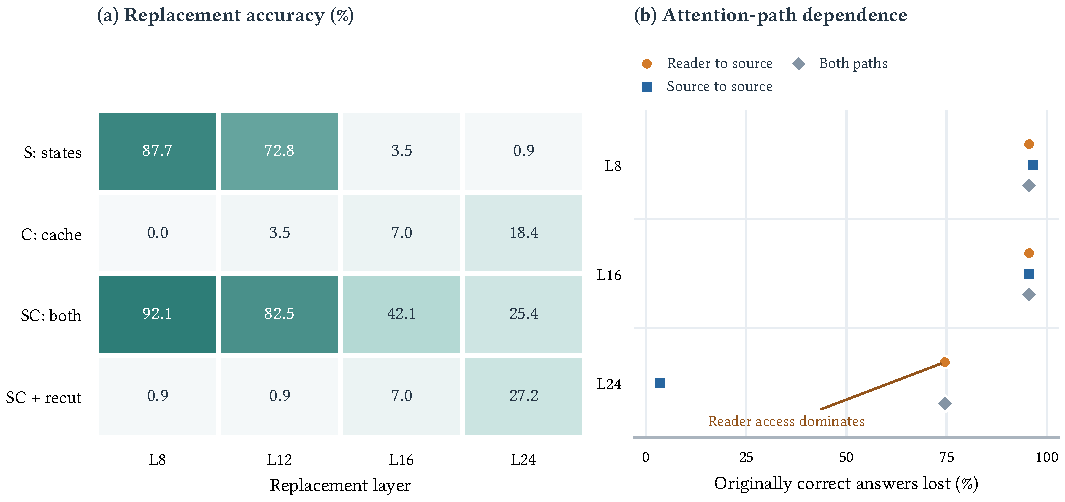
\includegraphics[width=\textwidth]{fig-mechanism-results.pdf}
\caption{Repair and attention-path results for all eight main combinations.
MC denotes MedCalc and TQA denotes TheoremQA. Each row uses its own fresh
split-prefill population; parentheses give questions/skill groups.
(a) Layer-16 accuracy after state ($S$), cache ($C$), joint ($SC$), or joint
replacement followed by a next-layer post-skill-to-skill recut.
(b) At layer 24, the fraction of donor-correct answers lost after cutting
post-skill-to-skill, skill-to-skill, or both paths. Both prefill and decoding
are intervened on. Table~\ref{tab:mechanism-contrasts} gives derived contrasts.}
\Description{Eight rows compare four repair accuracies at layer 16 and three attention-path losses at layer 24 across four models and two benchmarks.}
\label{fig:mechanism}
\end{figure*}
